\subsection{Date \& Time}

\begin{figure}[!ht]
 \centering
 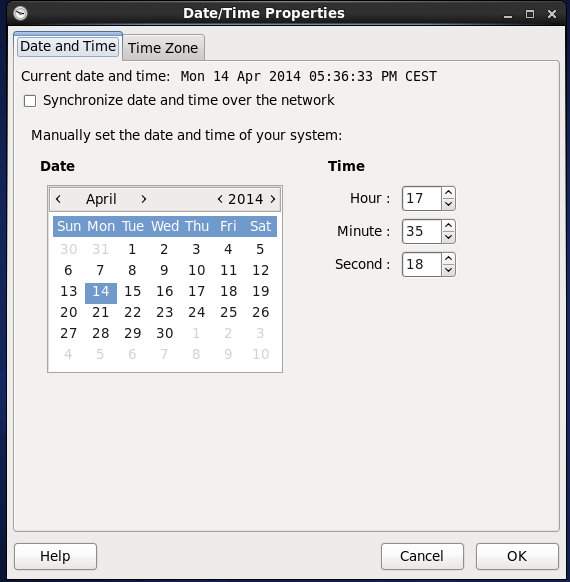
\includegraphics[scale=0.5]{Immagini/sys_conf_date1.png}
 \label{fig:System Config Date}
 \caption{system-config-date}
\end{figure}


L'utility di amministrazione ``Date \& Time'' visibile nel menu alla voce \menu{System > Administration > Date \& Time}, oppure richiamando direttamente l'applicazione \textit{system-config-date} permette la gestione di data ed ora, fuso orario e localizzazione geografica, consente di poter configurare il sistema alla interrogazione periodica di un server NTP in rete. 

Per l'uso di questa utility sono necessari i permessi di amministrazione.

%\textbf{System} $\rightarrow$ \textbf{Administration} $\rightarrow$ \textbf{Date \& Time})
\subsection{Printing}

\begin{figure}[!ht]
 \centering
 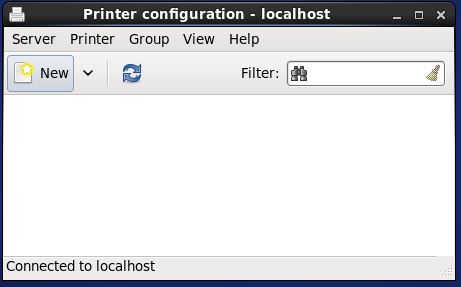
\includegraphics[scale=0.6]{Immagini/sys_conf_printing.png}
 \label{fig:System Config Printer}
 \caption{system-config-printer}
\end{figure}

L'utility di amministrazione ``Printing'', visibile nel menu alla voce \menu{System > Administration > Printig} oppure richiamando direttamente l'applicazione \textit{system-config-printer}, consente la configurazione delle stampanti di sistema, siano esse locali o remote. 

Per l'uso di questa utility sono necessari i permessi di amministrazione.

\subsection{User \& Groups}

\begin{figure}[!ht]
 \centering
 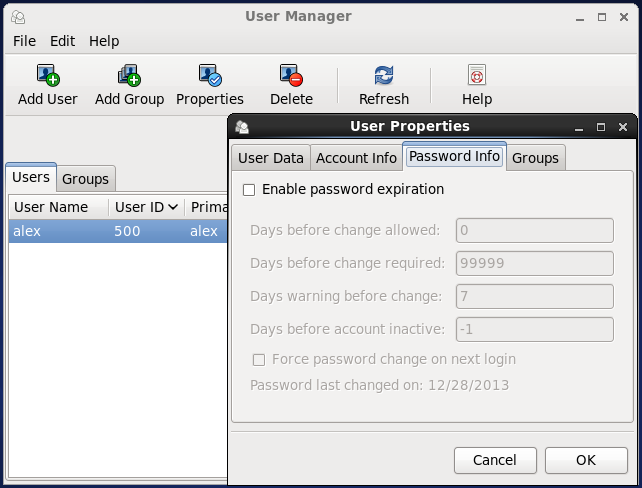
\includegraphics[scale=0.5]{Immagini/sys_conf_user1.png}
 \label{fig:System Config user}
 \caption{system-config-users}
\end{figure}




L'utility di amministazione ``User \& Groups'', visibile nel menù alla voce \menu{System > Administration > User \& Groups} oppure richiamando direttamente l'applicazione \textit{system-config-users}, consente la gestione e l'amministazione degli utenti del sistema, permettendo di poter lavorare contemporaneamente sulle informazione utente e su quelle di autenticazione. Ad esempio:

\begin{itemize}
 \item Creazione e rimozione utenti
 \item Creazione e rimozione gruppi
 \item Cambio password utenti
 \item Gestione gruppi secondari
 \item Account Expiration, Warning period e Password Expiration.
\end{itemize}


Per l'uso di questa utility sono necessari i permessi di amministrazione.